% mnras_template.tex
%
% LaTeX template for creating an MNRAS paper
%
% v3.0 released 14 May 2015
% (version numbers match those of mnras.cls)
%
% Copyright (C) Royal Astronomical Society 2015
% Authors:
% Keith T. Smith (Royal Astronomical Society)

% Change log
%
% v3.0 May 2015
%    Renamed to match the new package name
%    Version number matches mnras.cls
%    A few minor tweaks to wording
% v1.0 September 2013
%    Beta testing only - never publicly released
%    First version: a simple (ish) template for creating an MNRAS paper

%%%%%%%%%%%%%%%%%%%%%%%%%%%%%%%%%%%%%%%%%%%%%%%%%%
% Basic setup. Most papers should leave these options alone.
\documentclass[a4paper,fleqn,usenatbib]{mnras}

% MNRAS is set in Times font. If you don't have this installed (most LaTeX
% installations will be fine) or prefer the old Computer Modern fonts, comment
% out the following line
%\usepackage{newtxtext,newtxmath}
% Depending on your LaTeX fonts installation, you might get better results with one of these:
%\usepackage{mathptmx}
%\usepackage{txfonts}

% Use vector fonts, so it zooms properly in on-screen viewing software
% Don't change these lines unless you know what you are doing
\usepackage[T1]{fontenc}
\usepackage{ae,aecompl}


%%%%% AUTHORS - PLACE YOUR OWN PACKAGES HERE %%%%%

% Only include extra packages if you really need them. Common packages are:
\usepackage{graphicx}	% Including figure files
\usepackage{amsmath}	% Advanced maths commands
\usepackage{amssymb}	% Extra maths symbols

%%%%%%%%%%%%%%%%%%%%%%%%%%%%%%%%%%%%%%%%%%%%%%%%%%

%%%%% AUTHORS - PLACE YOUR OWN COMMANDS HERE %%%%%

% Please keep new commands to a minimum, and use \newcommand not \def to avoid
% overwriting existing commands. Example:
%\newcommand{\pcm}{\,cm$^{-2}$}	% per cm-squared

%%%%%%%%%%%%%%%%%%%%%%%%%%%%%%%%%%%%%%%%%%%%%%%%%%

%%%%%%%%%%%%%%%%%%% TITLE PAGE %%%%%%%%%%%%%%%%%%%

% Title of the paper, and the short title which is used in the headers.
% Keep the title short and informative.
\title[Short title, max. 45 characters]{MNRAS \LaTeXe\ template -- title goes here}

% The list of authors, and the short list which is used in the headers.
% If you need two or more lines of authors, add an extra line using \newauthor
\author[G. Chaparro-Molano et al.]{
Germ\'an Chaparro-Molano,$^{1}$\thanks{E-mail: gchaparrom@ecci.edu.co}
Juan Carlos Cuervo,$^{2}$
Oscar Alberto Restrepo Gait\'an$^{1,3}$
\\
% List of institutions
$^{1}$Vicerrector\'ia de Investigaci\'on, Universidad ECCI, 111311 Bogot\'a, Colombia\\
$^{2}$Department, Institution, Street Address, City Postal Code, Country\\
$^{3}$Radio Astronomy Instrumentation Group, Universidad de Chile, Santiago de Chile, Chile
}

% These dates will be filled out by the publisher
\date{Accepted XXX. Received YYY; in original form ZZZ}

% Enter the current year, for the copyright statements etc.
\pubyear{2015}

% Don't change these lines
\begin{document}
\label{firstpage}
\pagerange{\pageref{firstpage}--\pageref{lastpage}}
\maketitle

% Abstract of the paper
\begin{abstract}
This is a simple template for authors to write new MNRAS papers.
The abstract should briefly describe the aims, methods, and main results of the paper.
It should be a single paragraph not more than 250 words (200 words for Letters).
No references should appear in the abstract.
\end{abstract}

% Select between one and six entries from the list of approved keywords.
% Don't make up new ones.
\begin{keywords}
Galxies: distances -- keyword2 -- keyword3
\end{keywords}

%%%%%%%%%%%%%%%%%%%%%%%%%%%%%%%%%%%%%%%%%%%%%%%%%%

%%%%%%%%%%%%%%%%% BODY OF PAPER %%%%%%%%%%%%%%%%%%

\section{Introduction}

Efforts to reduce the uncertainty in the estimate the Hubble constant are single-method such as SNIa \citet{hubsn2018}. Bayesian analysis of systematic uncertainties for cosmology when using SNIa-derived galactic parameters (heterogeneous errors) \citet{unity}. Hubble constant MCMC estimation based on Cepheids distance determination for NGC 4258 \citet{hubngc}. \citet{hub2010} is the important hubble paper, although the original hubble estimation from redshift independent distances is \citet{huborig}. \citet{ridsn} estimates distances using snia but no redshifts. 

The \texttt{emcee} affine invariant MCMC ensemble sampler \citet{emcee} has been widely used due to its usability and efficiency. Markov Chain Monte Carlo (MCMC) samplers such as \citet{emcee} have been widely used for fitting data to models. Recently, \citet{propprob2018} used \texttt{emcee} for model assessment using Bayesian and Akaike Information Criteria along with Bayes factors, focusing on small datasets, where it is not relevant to reproduce the original variance of the data. \texttt{emcee} has also been proved to be useful in recovering probabilistic models for photometric redshifts \citet{photred1,photred2} . \citet{said} has used emcee for Tully-Fisher in the southern Zone of Avoidance.

Tully Fisher relation \citet{precisetf}

GW searches \citet{gwgallist}, we should improve redshift independent distance determination .

\citet{6df} attempt to predict redshift-derived distance errors within a Bayesian framework yields 26\%.

Exploration of prior discrepancy modeling in model estimation \citet{priordisc}

Importance of distance and catalogs \citet{catetg,catspi} in:

Other discrepancy measures for model selection \citet{otherdisc}. Chi2 model selection \citet{chi2ms}

The NASA/IPAC Extragalactic Distance (NED) catalog of Redshift-Independent Distances \citet{ned07,ned} is  a catalog with the following properties. HyperLEDA \citet{hyperleda} is a catalogue for extragalactic distances, which also includes redshift-independent distance measurements, but it is much smaller than NED. Extragalactic distance database \citet{distdb}. Changes in Hubble constant estimation using TF relation without Cepheids \citet{noceph}

Determining whether a galaxy belongs to a group by analyzing their common properties \citet{gg3500} 

Determining the spatial distribution of galaxies in order to study large-scale structure \citet{gallargescale} or local universe peculiar velocities \citet{localunipv}. Kinematics of nearby galaxies in void \citet{void}

Studies of anisotropy be it of morphological types \citet{morphanis} or density-velocity \citet{nongauss} which also need to take into account instrument detection limits \citet{catmatch} and source identification \citet{baymatch}. Anisotropy hubble from HST data \citet{anishub}

\citet{cosmicflows} distance errors are weighted standard deviations across different methods. Individual errors are not available for all methods. \citet{locunivcf} local universe structure reconstruction Cosmicflows-1

\citet{gmastro} is a widely used Bayesian linear regressor which uses a Gaussian Mixture Model to approximate the distibution of unobserved ``true'' data values and from this information estimate the regression coefficients.

10\% estimated uncertainty for photometrically derived distance scale ladder \citet{hubunc}

Are \citet{2mass} sources important in our analysis?

What I would like to know is what the TF method is. Also get better feeling of cosmicflows. Get better feeling of linmix fit. Do stuff to hyperleda catalog? Arm-wave my way out of that?

Remember that Cepheids and SNIa are primary distance indicators. TF FP are secondary 


\citet{tf07dist}



 \citet{chaparro18}, \citet{tecciencia}, \citet{gelmanppd} \citet{brooks} \citet{tforig}



This is a simple template for authors to write new MNRAS papers.
See \texttt{mnras\_sample.tex} for a more complex example, and \texttt{mnras\_guide.tex}
for a full user guide.

All papers should start with an Introduction section, which sets the work
in context, cites relevant earlier studies in the field by \citet{photred2},
and describes the problem the authors aim to solve \citep[e.g.][]{photred1}.

\section{Methods, Observations, Simulations etc.}

From here on, when we mention distance measurements in the NED-D catalog, we will be excluding from our analysis measurements that require the target redshift to calculate the distance, as indicated in the \texttt{redshift (z)} column.

In the NED-D database, $\sim16000$ galaxies ($\sim9$\%) have more than one distance measurement, $\sim1800$ galaxies ($\sim1$\%) have more than 12  distance measurements, and $~180$ galaxies ($\sim0.1$\%) have distances measurements using more than 6 different methods. \\

For many galaxies, the random error for each measurement is not representative of the scatter across different measurements, even when considering measurements that use the same method. In addition, distance modulus distributions for each measurement (which are assumed to be Gaussian) are transformed to log-normal distributions in distance space. For this reason, we consider that the best approach to consider the effects of random and scattering errors in catalog-wide, multi-method distance analyses is to take bootstrap samples of the posterior distribution for each extragalactic distance. The posterior distribution can be obtained by drawing distance samples from the mixture of the log-normal distributions corresponding to each measurement.\\

However, the previous approach, while thorough, is not very efficient

Normally the next section describes the techniques the authors used.
It is frequently split into subsections, such as Section~\ref{sec:maths} below.

\subsection{Maths}
\label{sec:maths} % used for referring to this section from elsewhere

Simple mathematics can be inserted into the flow of the text e.g. $2\times3=6$
or $v=220$\,km\,s$^{-1}$, but more complicated expressions should be entered
as a numbered equation:

\begin{equation}
    x=\frac{-b\pm\sqrt{b^2-4ac}}{2a}.
	\label{eq:quadratic}
\end{equation}

Refer back to them as e.g. equation~(\ref{eq:quadratic}).

\subsection{Figures and tables}

Figures and tables should be placed at logical positions in the text. Don't
worry about the exact layout, which will be handled by the publishers.

Figures are referred to as e.g. Fig.~\ref{fig:example_figure}, and tables as
e.g. Table~\ref{tab:example_table}.

% Example figure
\begin{figure}
	% To include a figure from a file named example.*
	% Allowable file formats are eps or ps if compiling using latex
	% or pdf, png, jpg if compiling using pdflatex
	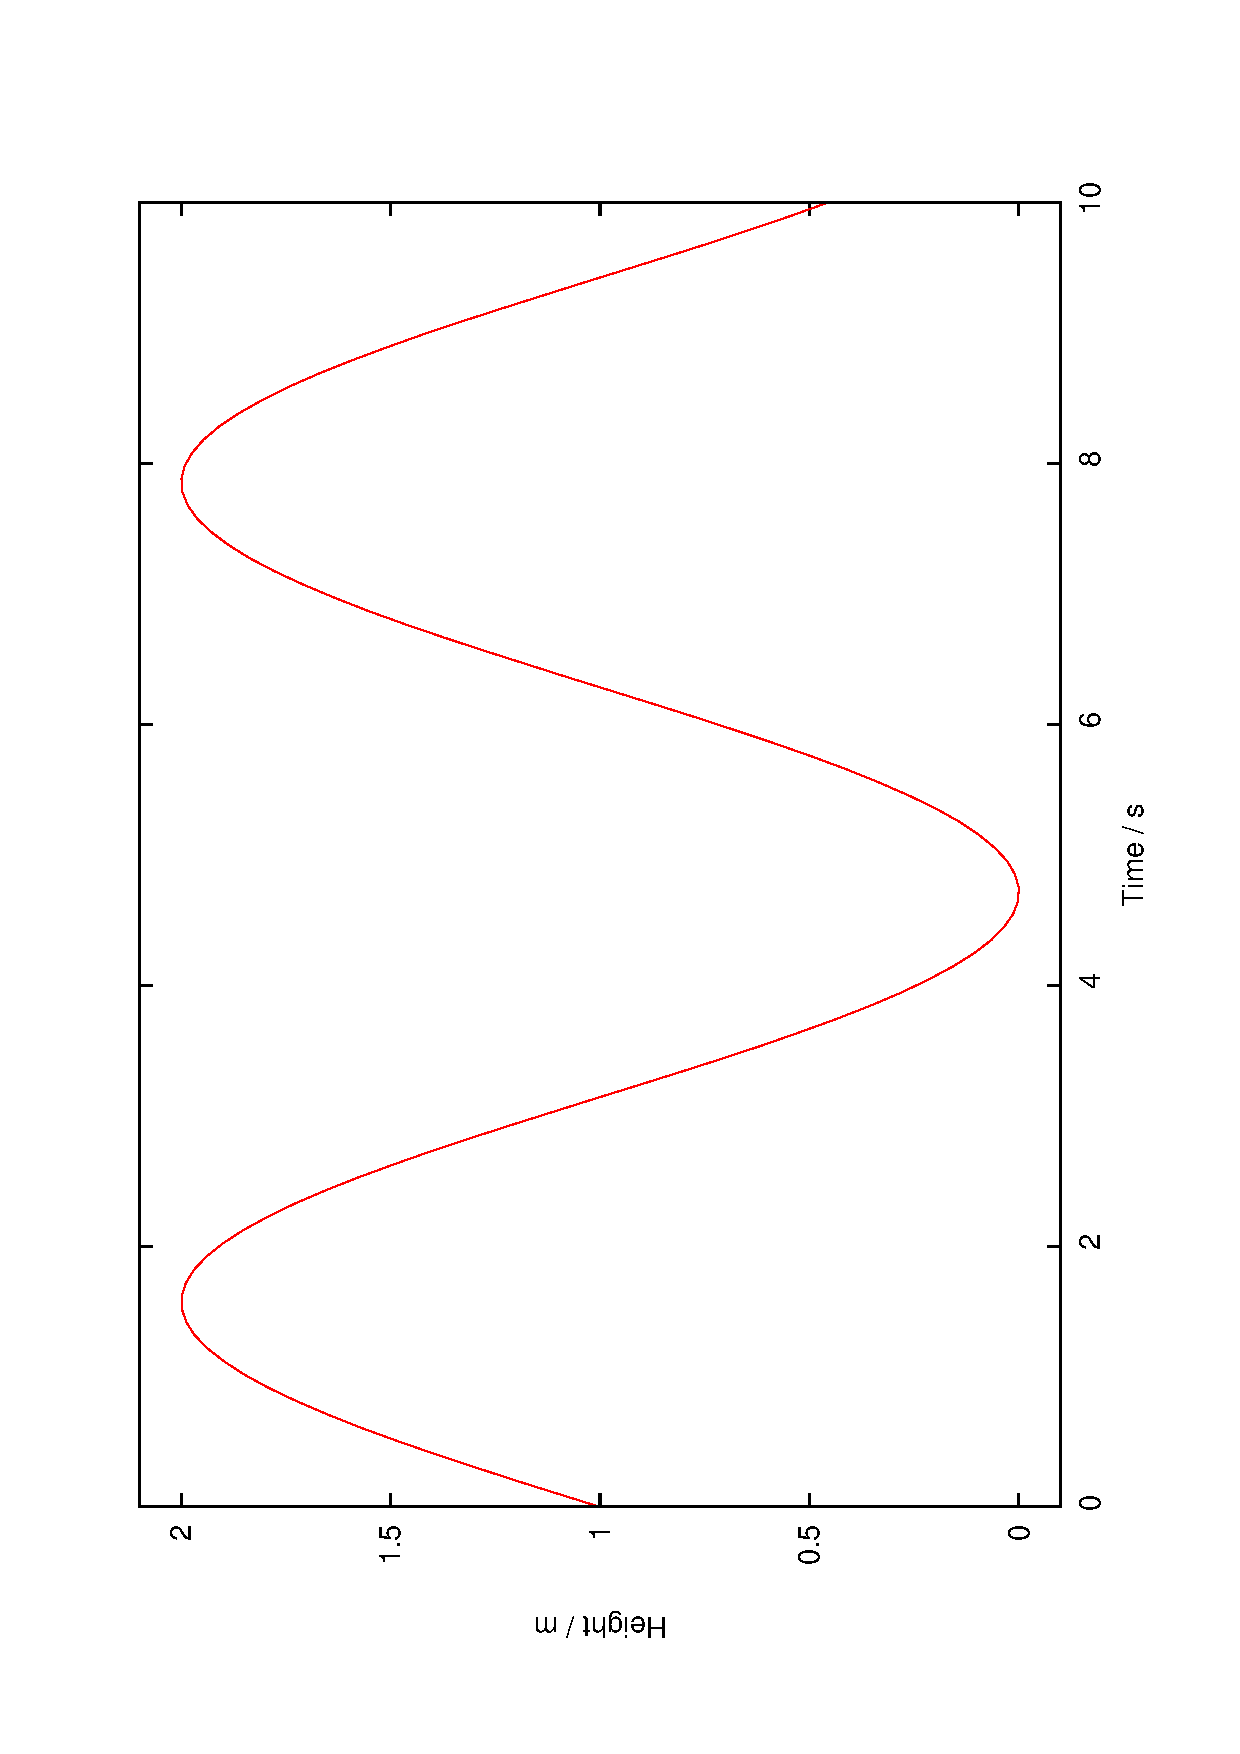
\includegraphics[width=\columnwidth]{example}
    \caption{This is an example figure. Captions appear below each figure.
	Give enough detail for the reader to understand what they're looking at,
	but leave detailed discussion to the main body of the text.}
    \label{fig:example_figure}
\end{figure}

% Example table
\begin{table}
	\centering
	\caption{This is an example table. Captions appear above each table.
	Remember to define the quantities, symbols and units used.}
	\label{tab:example_table}
	\begin{tabular}{lccr} % four columns, alignment for each
		\hline
		A & B & C & D\\
		\hline
		1 & 2 & 3 & 4\\
		2 & 4 & 6 & 8\\
		3 & 5 & 7 & 9\\
		\hline
	\end{tabular}
\end{table}


\section{Conclusions}

The last numbered section should briefly summarise what has been done, and describe
the final conclusions which the authors draw from their work.

\section*{Acknowledgements}

The Acknowledgements section is not numbered. Here you can thank helpful
colleagues, acknowledge funding agencies, telescopes and facilities used etc.
Try to keep it short.

%%%%%%%%%%%%%%%%%%%%%%%%%%%%%%%%%%%%%%%%%%%%%%%%%%

%%%%%%%%%%%%%%%%%%%% REFERENCES %%%%%%%%%%%%%%%%%%

% The best way to enter references is to use BibTeX:

\bibliographystyle{mnras}
\bibliography{savedrecs} % if your bibtex file is called example.bib


% Alternatively you could enter them by hand, like this:
% This method is tedious and prone to error if you have lots of references
%\begin{thebibliography}{99}
%\bibitem[\protect\citeauthoryear{Author}{2012}]{Author2012}
%Author A.~N., 2013, Journal of Improbable Astronomy, 1, 1
%\bibitem[\protect\citeauthoryear{Others}{2013}]{Others2013}
%Others S., 2012, Journal of Interesting Stuff, 17, 198
%\end{thebibliography}

%%%%%%%%%%%%%%%%%%%%%%%%%%%%%%%%%%%%%%%%%%%%%%%%%%

%%%%%%%%%%%%%%%%% APPENDICES %%%%%%%%%%%%%%%%%%%%%

\appendix

\section{Some extra material}

If you want to present additional material which would interrupt the flow of the main paper,
it can be placed in an Appendix which appears after the list of references.

%%%%%%%%%%%%%%%%%%%%%%%%%%%%%%%%%%%%%%%%%%%%%%%%%%


% Don't change these lines
\bsp	% typesetting comment
\label{lastpage}
\end{document}

% End of mnras_template.tex